\documentclass[a4paper,12pt,twoside]{memoir}

% Castellano
\usepackage[spanish,es-tabla]{babel}
\selectlanguage{spanish}
\usepackage[utf8]{inputenc}
\usepackage[T1]{fontenc}
\usepackage{lmodern} % scalable font
\usepackage{microtype}
\usepackage{placeins}

\usepackage{eurosym}
\usepackage{longtable,booktabs}

% Bibliography management
\usepackage[numbers,sort]{natbib}

\RequirePackage{booktabs}
\RequirePackage[table]{xcolor}
\RequirePackage{xtab}
\RequirePackage{multirow}

% Links
\usepackage[colorlinks]{hyperref}
\hypersetup{
	allcolors = {blue}
}

% Ecuaciones
\usepackage{amsmath}

% Rutas de fichero / paquete
\newcommand{\ruta}[1]{{\sffamily #1}}

% Párrafos
\nonzeroparskip


% Imagenes
\usepackage{graphicx}
\newcommand{\imagen}[2]{
	\begin{figure}[!h]
		\centering
		\includegraphics[width=0.9\textwidth]{#1}
		\caption{#2}\label{fig:#1}
	\end{figure}
	\FloatBarrier
}

\newcommand{\imagenflotante}[2]{
	\begin{figure}%[!h]
		\centering
		\includegraphics[width=0.9\textwidth]{#1}
		\caption{#2}\label{fig:#1}
	\end{figure}
}



% El comando \figura nos permite insertar figuras comodamente, y utilizando
% siempre el mismo formato. Los parametros son:
% 1 -> Porcentaje del ancho de página que ocupará la figura (de 0 a 1)
% 2 --> Fichero de la imagen
% 3 --> Texto a pie de imagen
% 4 --> Etiqueta (label) para referencias
% 5 --> Opciones que queramos pasarle al \includegraphics
% 6 --> Opciones de posicionamiento a pasarle a \begin{figure}
\newcommand{\figuraConPosicion}[6]{%
  \setlength{\anchoFloat}{#1\textwidth}%
  \addtolength{\anchoFloat}{-4\fboxsep}%
  \setlength{\anchoFigura}{\anchoFloat}%
  \begin{figure}[#6]
    \begin{center}%
      \Ovalbox{%
        \begin{minipage}{\anchoFloat}%
          \begin{center}%
            \includegraphics[width=\anchoFigura,#5]{#2}%
            \caption{#3}%
            \label{#4}%
          \end{center}%
        \end{minipage}
      }%
    \end{center}%
  \end{figure}%
}

%
% Comando para incluir imágenes en formato apaisado (sin marco).
\newcommand{\figuraApaisadaSinMarco}[5]{%
  \begin{figure}%
    \begin{center}%
    \includegraphics[angle=90,height=#1\textheight,#5]{#2}%
    \caption{#3}%
    \label{#4}%
    \end{center}%
  \end{figure}%
}
% Para las tablas
\newcommand{\otoprule}{\midrule [\heavyrulewidth]}
%
% Nuevo comando para tablas pequeñas (menos de una página).
\newcommand{\tablaSmall}[5]{%
 \begin{table}
  \begin{center}
   \rowcolors {2}{gray!35}{}
   \begin{tabular}{#2}
    \toprule
    #4
    \otoprule
    #5
    \bottomrule
   \end{tabular}
   \caption{#1}
   \label{tabla:#3}
  \end{center}
 \end{table}
}

%
%Para el float H de tablaSmallSinColores
\usepackage{float}

%
% Nuevo comando para tablas pequeñas (menos de una página).
\newcommand{\tablaSmallSinColores}[5]{%
 \begin{table}[H]
  \begin{center}
   \begin{tabular}{#2}
    \toprule
    #4
    \otoprule
    #5
    \bottomrule
   \end{tabular}
   \caption{#1}
   \label{tabla:#3}
  \end{center}
 \end{table}
}

\newcommand{\tablaApaisadaSmall}[5]{%
\begin{landscape}
  \begin{table}
   \begin{center}
    \rowcolors {2}{gray!35}{}
    \begin{tabular}{#2}
     \toprule
     #4
     \otoprule
     #5
     \bottomrule
    \end{tabular}
    \caption{#1}
    \label{tabla:#3}
   \end{center}
  \end{table}
\end{landscape}
}

%
% Nuevo comando para tablas grandes con cabecera y filas alternas coloreadas en gris.
\newcommand{\tabla}[6]{%
  \begin{center}
    \tablefirsthead{
      \toprule
      #5
      \otoprule
    }
    \tablehead{
      \multicolumn{#3}{l}{\small\sl continúa desde la página anterior}\\
      \toprule
      #5
      \otoprule
    }
    \tabletail{
      \hline
      \multicolumn{#3}{r}{\small\sl continúa en la página siguiente}\\
    }
    \tablelasttail{
      \hline
    }
    \bottomcaption{#1}
    \rowcolors {2}{gray!35}{}
    \begin{xtabular}{#2}
      #6
      \bottomrule
    \end{xtabular}
    \label{tabla:#4}
  \end{center}
}

%
% Nuevo comando para tablas grandes con cabecera.
\newcommand{\tablaSinColores}[6]{%
  \begin{center}
    \tablefirsthead{
      \toprule
      #5
      \otoprule
    }
    \tablehead{
      \multicolumn{#3}{l}{\small\sl continúa desde la página anterior}\\
      \toprule
      #5
      \otoprule
    }
    \tabletail{
      \hline
      \multicolumn{#3}{r}{\small\sl continúa en la página siguiente}\\
    }
    \tablelasttail{
      \hline
    }
    \bottomcaption{#1}
    \begin{xtabular}{#2}
      #6
      \bottomrule
    \end{xtabular}
    \label{tabla:#4}
  \end{center}
}

%
% Nuevo comando para tablas grandes sin cabecera.
\newcommand{\tablaSinCabecera}[5]{%
  \begin{center}
    \tablefirsthead{
      \toprule
    }
    \tablehead{
      \multicolumn{#3}{l}{\small\sl continúa desde la página anterior}\\
      \hline
    }
    \tabletail{
      \hline
      \multicolumn{#3}{r}{\small\sl continúa en la página siguiente}\\
    }
    \tablelasttail{
      \hline
    }
    \bottomcaption{#1}
  \begin{xtabular}{#2}
    #5
   \bottomrule
  \end{xtabular}
  \label{tabla:#4}
  \end{center}
}



\definecolor{cgoLight}{HTML}{EEEEEE}
\definecolor{cgoExtralight}{HTML}{FFFFFF}

%
% Nuevo comando para tablas grandes sin cabecera.
\newcommand{\tablaSinCabeceraConBandas}[5]{%
  \begin{center}
    \tablefirsthead{
      \toprule
    }
    \tablehead{
      \multicolumn{#3}{l}{\small\sl continúa desde la página anterior}\\
      \hline
    }
    \tabletail{
      \hline
      \multicolumn{#3}{r}{\small\sl continúa en la página siguiente}\\
    }
    \tablelasttail{
      \hline
    }
    \bottomcaption{#1}
    \rowcolors[]{1}{cgoExtralight}{cgoLight}

  \begin{xtabular}{#2}
    #5
   \bottomrule
  \end{xtabular}
  \label{tabla:#4}
  \end{center}
}




\graphicspath{ {./img/} }

% Capítulos
\chapterstyle{bianchi}
\newcommand{\capitulo}[2]{
	\setcounter{chapter}{#1}
	\setcounter{section}{0}
	\chapter*{#2}
	\addcontentsline{toc}{chapter}{#2}
	\markboth{#2}{#2}
}

% Apéndices
\renewcommand{\appendixname}{Apéndice}
\renewcommand*\cftappendixname{\appendixname}

\newcommand{\apendice}[1]{
	%\renewcommand{\thechapter}{A}
	\chapter{#1}
}

\renewcommand*\cftappendixname{\appendixname\ }

% Formato de portada
\makeatletter
\usepackage{xcolor}
\newcommand{\tutor}[1]{\def\@tutor{#1}}
\newcommand{\course}[1]{\def\@course{#1}}
\definecolor{cpardoBox}{HTML}{E6E6FF}
\def\maketitle{
  \null
  \thispagestyle{empty}
  % Cabecera ----------------
\noindent
\includegraphics[width=\textwidth]{cabecera}\vspace{1cm}%
  \vfill
  % Título proyecto y escudo informática ----------------
  \colorbox{cpardoBox}{%
    \begin{minipage}{.8\textwidth}
      \vspace{.5cm}\Large
      \begin{center}
      \textbf{TFG del Grado en Ingeniería Informática}\vspace{.6cm}\\
      \textbf{\LARGE\@title{}}
      \end{center}
      \vspace{.2cm}
    \end{minipage}

  }%
  \hfill\begin{minipage}{.20\textwidth}
    
\includegraphics[width=\textwidth]{escudoInfor}
  \end{minipage}
  \vfill
  % Datos de alumno, curso y tutores ------------------
  \begin{center}%
  {%
    \noindent\LARGE
    Presentado por \@author{}\\ 
    en Universidad de Burgos --- \@date{}\\
    Tutor: \@tutor{}\\
  }%
  \end{center}%
  \null
  \cleardoublepage
  }
\makeatother


% Datos de portada
\title{PCVN \\Documentación Técnica}
\author{Roberto Poza Puras}
\tutor{Dr.César Ignacio García Osorio \\ y Dr. Juan Jose Rodriguez Diez}
\date{\today}

\begin{document}

\maketitle



\cleardoublepage



%%%%%%%%%%%%%%%%%%%%%%%%%%%%%%%%%%%%%%%%%%%%%%%%%%%%%%%%%%%%%%%%%%%%%%%%%%%%%%%%%%%%%%%%



\frontmatter


\clearpage

% Indices
\tableofcontents

\clearpage

\listoffigures

\clearpage

\listoftables

\clearpage

\mainmatter

\appendix

\apendice{Plan de Proyecto Software}

\section{Introducción}
La fase de planificación es uno de los pilares fundamentales de cualquier proyecto, en esta fase se determinan los objetivos, el tiempo y el dinero que va a suponer la realización del proyecto. Así pues, vamos a dividir la fase de planificación en:
\begin{itemize}
	\item Planificación temporal
	\item Estudio de viabilidad
\end{itemize}
\section{Planificación temporal}
En el desarrollo del proyecto se planteó utilizar una metodología de trabajo basado en el desarrollo ágil, para ello se utilizó la metodología \emph{Scrum}.
\begin{itemize}
	\item Se aplicó una estrategia de desarrollo incremental basada en \emph{sprints}
	\item La duración de los \emph{sprints} fue de una semana.
	\item Al inicio del \emph{sprint} se definían los objetivos a alcanzar.
	\item Al final del \emph{sprint} se revisa los objetivos conseguidos y los problemas encontrados.
\end{itemize}
A continuación, se van a describir \emph{sprints} que se han realizado.

\subsection{Sprint 0 (5/11/18 - 11/11/18)}
En la primera reunión de planificación de proyecto se sentaron las ideas del mismo y se marcaron los objetivos de este \textbf{primer \emph{sprint}}.

Los objetivos concretados de este primer \emph{sprint} fueron:
\begin{itemize}
	\item Realizar una toma de contacto con las distintas páginas web, así como con las técnicas de \emph{Web Scarping} y las bibliotecas sugeridas para trabajar.
	\item La creación formal del repositorio sobre el que se está trabajando actualmente. Para un mejor uso el tutor recomendó la adquisición del \emph{Github Student Developer Pack} ,el cual fue solicitado y ha sido ya recibido, permitiendo entre otras muchas cosas el uso de los repositorios privados.
\end{itemize}
Además, proporcionó numerosos enlaces sobre \emph{Web Scarping} que formarán parte de la toma de contacto y un posterior aprendizaje más profundo.

Se estiman 9 horas de trabajo
\subsection{Sprint 1 (12/11/18 - 18/11/18)}
Los objetivos determinados para este \textbf{segundo \emph{sprint}} han sido : 
\begin{itemize}
\item investigar los tipos de formatos posibles para procesado de los datos extraídos de las distintas fuentes.
\end{itemize}
Se sugirieron los siguentes formatos:
\begin{itemize}
\item \emph{Bibtex}
\item \emph{RIS}
\item \emph{EndNote}
\end{itemize}
Se estiman 20 horas de trabajo.

\subsection{Sprint 2 (19/11/18 - 25/11/18)}
Los objetivos determinados para este \textbf{tercer \emph{sprint}} han sido:
\begin{itemize}
	\item Implementación del formato \emph{BibTex}, como forma de devolver los datos. Para un posterior Procesado.
\end{itemize}

Se estiman 20 horas de trabajo.

\subsection{Sprint 3 (26/11/18 - 1/12/18)}
Los objetivos determinados para este \textbf{cuarto \emph{sprint}} han sido:
\begin{itemize}
	\item La documentación acerca de \LaTeX, con el fin de comenzar con el desarrollo de la memoria del proyecto y poder 
	 realizar una documentación detallada del desarrollo del proyecto.
	 \item Solucionar algunos problemas referentes a la obtención de los datos con los scripts publicados en los anteriores \emph{sprints}.
\end{itemize}

Se estiman 30 horas de trabajo
\subsection{Sprint 4 (3/12/18 - 9/12/18)}

Los objetivos determinados para este \textbf{quinto \emph{sprint}} han sido:
\begin{itemize}
	\item Estudiar el funcionamiento de la aplicación de la \textbf{\emph{ANECA}}, con el fin de realizar un script que permita la automatización de la subida de los datos extraídos del resto de páginas.
\end{itemize}

Se estiman 30 horas de trabajo

Finalmente se desarrolló la estructura básica para el acceso a la \emph{ANECA} y un script para la eliminación de duplicados y agrupamiento de los ficheros \emph{BibTeX} llamado GroupFiles. 

Con un total de 30.5 horas de trabajo
\subsection{Sprint 5 (10/12/18 - 16/12/18)}

Los objetivos determinados para este \textbf{sexto \emph{sprint}} han sido:
\begin{itemize}
	\item Implementar el script para la automatización de la subida de los datos bibliográficos extraídos.
\end{itemize}

Se estiman 25 horas de trabajo

Finalmente se tuvieron que realizar cambios en el script dedicado a la eliminación de elementos duplicados
y agrupación de ficheros, pues se producían errores en el proceso de automatización. Se mejoro el sistema de comparación de publicaciones (añadiendo comparación por ISSN).
El script de automatización quedo sin terminar, quedando pendiente la depuración de errores.


Se emplearon 28.5 horas de trabajo
\subsection{Sprint 6 (17/12/18 - 23/12/18)}
Los objetivos determinados para este \textbf{séptimo \emph{sprint}} han sido:
\begin{itemize}
	\item Depuración de errores del script de automatización de subida de los datos bibliográficos extraídos.
	\item Extraer índice de impacto de las publicaciones correspondientes de Web of Science.
	\item Añadir funcionalidad para identificar y subir los artículos con índice de impacto.
	\item Introducción a las librerías y métodos más usuales para desarrollar una interfaz Gráfica.
\end{itemize}

Se estiman 30 horas de trabajo

\textbf{Finalmente se invirtieron 29.5 horas}
\subsection{Sprint 7 (24/12/18 - 30/12/18)}
Los objetivos determinados para este \textbf{octavo \emph{sprint}} han sido:
\begin{itemize}
	\item Implementar una interfaz gráfica dotando al proyecto de una estructura más sólida y amigable para el usuario final.
	\item Implementar funcionalidad que notifique al usuario de aquellas publicaciones que no se hayan podido subir a \emph{ANECA} guardándolo en un fichero \emph{BibTeX}, para que sea el propio usuario quien decida qué hacer con ello.
	\item Adaptar el código a formato \emph{PEP8}
\end{itemize}

Se estiman 30 horas de trabajo

Finalmente se emplearon 32.5 horas de trabajo pendiente de terminar la adaptación al formato \emph{PEP8} del código, así como algunos errores de poca importancia
\subsection{Sprint 8 (31/12/18 - 6/1/19)}

Los objetivos determinados para este \textbf{noveno \emph{sprint}} han sido:
\begin{itemize}
	\item Finalizar las tareas pendientes del \emph{sprint 7.}
	\item Implementar Unit Test, para mejorar la robustez del código.
\end{itemize}
Se estiman 15 horas de trabajo.

Se finalizaron las tareas pendientes de realizar del \emph{sprint 7}, además se añadieron nuevas herramientas para permitir la extracción de nuevos indicios de calidad de las publicaciones.
Empleando un Total de 26.5 horas y quedando pendiente la implementación de los Unit Test
\subsection{Sprint 9 (7/1/19 - 13/1/19)}
Los objetivos determinados para este \textbf{décimo \emph{sprint}} han sido:
\begin{itemize}
	\item Finalizar las tareas pendientes del sprint 8.
	\item Tratar las excepciones generadas y permitiendo la recuperación del programa cuando una ocurra.
\end{itemize}
Se estiman 25 horas de Trabajo.

\begin{itemize}
	\item Tras un error en la \emph{API} que proporcionaba acceso a los datos de \emph{Scopus} y que hace inviable seguir utilizando este método (pues no devolvía los autores de las publicaciones), se decide cambiar el actual método para pasar a utilizar la herramienta \emph{Selenium} (tras una previa investigación). Mejorando los tiempos de ejecución.
	\item Numerosas excepciones generadas y errores de carga por parte de \emph{Selenium} han ralentizado el desarrollo de los objetivos marcados para este \emph{sprint}, se comienza el domingo 13/1/19 a evaluar posibles alternativas a \emph{Selenium}.
\end{itemize}

Empleadas 25 horas de trabajo sin avance en los objetivos iniciales del \emph{sprint}, los nuevos objetivos fueron finalizados con éxito.
\begin{itemize}
	\item Implementar la extracción de datos de  \emph{Scopus} mediante el uso de \emph{Selenium}.
	\item Investigar una nueva forma de acceder a ACADEMIA para realizar la subida de las publicaciones sin necesidad de usar \emph{Selenium}
\end{itemize}

\subsection{Sprint 10 (14/1/19 - 20/1/19)}
Los objetivos determinados para este \textbf{undécimo \emph{sprint}} han sido:
\begin{itemize}
	\item Finalizar las tareas pendientes del \emph{sprint 9}.
		\begin{itemize}
			\item Implementar Unit Test, para mejorar la robustez del código.
			\item Tratar las excepciones generadas y permitiendo la recuperación del programa cuando una ocurra.
		\end{itemize}
	\item Encontrar alternativa al uso de \emph{Selenium} para la inyección de datos en ACADEMIA.
	\item Probar la robustez de la aplicación.
\end{itemize}

\emph{Se estiman 30 horas de Trabajo.}

El martes se toma la decisión, de manejar las peticiones \emph{GET} y \emph{POST} directamente mediante el uso de la librería para Python: \emph{requests}.
\subsection{Sprint 11 (21/1/19 - 27/1/19)}
Los objetivos determinados para este \emph{duodécimo sprint} han sido:
\begin{itemize}
	\item Seguir con las labores de documentación iniciadas el sprint 3.
	\item Probar la robustez de la aplicación y corregir errores encontrados.
	\item Mejorar la interacción del usuario con la interfaz gráfica.
\end{itemize}
Se estiman 20 horas de trabajo.

\subsection{Sprint 12 (28/1/19 - 3/2/19)}
Los objetivos determinados para este \emph{decimotercer sprint} han sido:
\begin{itemize}
	\item Continuar con las labores iniciadas en el sprint anterior, con el fin mejorar la experiencia del usuario y la funcionalidad de la aplicación.
\end{itemize}
Se estiman 18 horas de trabajo.

\subsection{Sprint 13 (4/2/19 - 10/2/19)}
Los objetivos determinados para este \emph{decimocuarto sprint} han sido:
\begin{itemize}
	\item Corregir errores de funcionalidad descubiertos en el anterior sprint.
	\item Implementar esperas adaptativas para los ficheros en los que se usa Selenium.
	\item Mejorar el uso de manejadores de Layouts.
	\item Capturar todas las excepciones para que la aplicación pueda recuperarse e informar al usuario de lo ocurrido.
	\item Implementar ventanas emergentes para informar al usuario de los errores en lugar de los cuadros de texto que hasta ahora se estaban utilizando.
\end{itemize}
Se estima 35 horas de trabajo. \\
Durante el trascurso de este sprint se han implementado los objetivos arriba descritos y corregido algunos errores encontrados durante las pruebas que se han realizado. Además, se ha implementado las siguientes funcionalidades:
\begin{itemize}
	\item Funcionalidad que permite elegir que partes del proceso se desean llevar a cabo.
	\item Funcionalidad que permite limitar el número de publicaciones a recuperar.
	\item Funcionalidad que permite guardar los errores en fichero para los usuarios avanzados.
	\item Funcionalidad que permite ver los archivos con las publicaciones extraídas o las subidas.
	\item Finalmente se han invertido un total de 37 horas.
\end{itemize}
Se estiman 20 horas de trabajo.

\subsection{Gráficos y Estadísticas}
Basándonos en los datos ofrecidos por GitHub se va a mostrar una serie de imágenes acerca del desarrollo del proyecto.
\begin{itemize}
	\item Commits: en la siguiente gráfica de barras se muestra por semanas la cantidad de commits que se han realizado.
	\item Añadidos y eliminados: En la siguiente gráfica se muestra la cantidad de líneas añadidas (entre todos los ficheros) y la cantidad de líneas eliminadas. Como podemos observar existe una gran cantidad de líneas eliminadas y esto se debe a los cambios de herramienta y/o procedimiento que han sido necesario llevar a cabo.\\En esta última fotografía vemos el total de líneas añadidas y eliminadas.
	[FOTO líneas de code]

\end{itemize}

\section{Estudio de viabilidad}
\subsection{Viabilidad Económica}
En este apartado vamos a realizar un supuesto de los costes y beneficios que hubiera tenido el desarrollo de este proyecto en un entorno empresarial real.\\
\textbf{Costes}\\
Podemos dividir la estructura de costes en dos categorías 
\begin{itemize}
	\item \textbf{Coste Material}
	En este apartado vamos a hacer dos diferencias:
	\begin{itemize}
		\item \emph{Hardware}: Para la realización del proyecto, se ha utilizado exclusivamente un ordenador portátil valorado en 850 \euro{} al cual se le estima un tiempo de amortización de cinco años y el tiempo que ha sido utilizado tres meses.
		
\begin{longtable}[]{@{}lrr@{}}
\toprule
\begin{minipage}[b]{0.29\columnwidth}\raggedright\strut
\textbf{Concepto}\strut
\end{minipage} & \begin{minipage}[b]{0.18\columnwidth}\raggedright\strut
\textbf{Coste}\strut
\end{minipage} & \begin{minipage}[b]{0.32\columnwidth}\raggedright\strut
\textbf{Coste amortizado}\strut
\end{minipage}\tabularnewline
\midrule
\endhead
\begin{minipage}[t]{0.29\columnwidth}\raggedright\strut
Ordenador portátil\strut
\end{minipage} & \begin{minipage}[t]{0.18\columnwidth}\raggedright\strut
850\euro{}\strut
\end{minipage} & \begin{minipage}[t]{0.32\columnwidth}\raggedright\strut
42.5\euro{}\strut
\end{minipage}\tabularnewline
\midrule
\begin{minipage}[t]{0.29\columnwidth}\raggedright\strut
\end{minipage}\tabularnewline

\caption{Costes de \emph{hardware}.}
\end{longtable}
		\item \emph{Software}: Para la realización del proyecto se han utilizado casi en su totalidad herramientas de uso libre y gratuito, la única herramienta de software no gratuita es el IDE de \emph{JetBrains}, el cual se ha utilizado con licencia de estudiante, pero dado que se trata de un supuesto de entorno empresarial se necesitaría una licencia adecuada para ello. El coste de la licencia es anual por ello se considera el tiempo de amortización de un año y el tiempo de uso de 3 meses. 
	\end{itemize}
	\begin{longtable}[]{@{}lrr@{}}
\toprule
\begin{minipage}[b]{0.29\columnwidth}\raggedright\strut
\textbf{Concepto}\strut
\end{minipage} & \begin{minipage}[b]{0.18\columnwidth}\raggedright\strut
\textbf{Coste}\strut
\end{minipage} & \begin{minipage}[b]{0.32\columnwidth}\raggedright\strut
\textbf{Coste amortizado}\strut
\end{minipage}\tabularnewline
\midrule
\endhead
\begin{minipage}[t]{0.29\columnwidth}\raggedright\strut
\emph{JetBrains PyCharm}\strut
\end{minipage} & \begin{minipage}[t]{0.18\columnwidth}\raggedright\strut
89\euro{}\strut
\end{minipage} & \begin{minipage}[t]{0.32\columnwidth}\raggedright\strut
22,25\euro{}\strut
\end{minipage}\tabularnewline
\midrule
\begin{minipage}[t]{0.29\columnwidth}\raggedright\strut
\end{minipage}\tabularnewline

\caption{Costes de \emph{software}.}
\end{longtable}

	\item \textbf{Coste Personal}
	El proyecto ha sido llevado a cabo por un desarrollador junior a tiempo completo durante un total de 3 meses. Se considera así los siguientes costes:
	\begin{longtable}[]{@{}lr@{}}
\toprule
\begin{minipage}[b]{0.38\columnwidth}\raggedright\strut
\textbf{Concepto}\strut
\end{minipage} & \begin{minipage}[b]{0.20\columnwidth}\raggedright\strut
\textbf{Coste}\strut
\end{minipage}\tabularnewline
\midrule
\endhead
\begin{minipage}[t]{0.38\columnwidth}\raggedright\strut
Salario mensual neto\strut
\end{minipage} & \begin{minipage}[t]{0.20\columnwidth}\raggedright\strut
1.000\euro{}\strut
\end{minipage}\tabularnewline
\begin{minipage}[t]{0.38\columnwidth}\raggedright\strut
Retención IRPF (15\%)\strut
\end{minipage} & \begin{minipage}[t]{0.20\columnwidth}\raggedright\strut
272,23\euro{}\strut
\end{minipage}\tabularnewline
\begin{minipage}[t]{0.38\columnwidth}\raggedright\strut
Seguridad Social (29,9\%)\strut
\end{minipage} & \begin{minipage}[t]{0.20\columnwidth}\raggedright\strut
542,65\euro{}\strut
\end{minipage}\tabularnewline
\begin{minipage}[t]{0.38\columnwidth}\raggedright\strut
Salario mensual bruto\strut
\end{minipage} & \begin{minipage}[t]{0.20\columnwidth}\raggedright\strut
1.814,88\euro{}\strut
\end{minipage}\tabularnewline
\midrule
\begin{minipage}[t]{0.38\columnwidth}\raggedright\strut
\textbf{Total 3 meses}\strut
\end{minipage} & \begin{minipage}[t]{0.20\columnwidth}\raggedright\strut
2.900,18 \euro{}\strut
\end{minipage}\tabularnewline
\bottomrule
\caption{Costes de personal.}
\end{longtable}

Se ha calculado la retribución a la Seguridad Social como un 29,9\% : 
\begin{itemize}
	\item 23,6\% por contingencias comunes.
	\item 5,5\% desempleo de tipo general.
	\item 0,6\% formación profesional.
	\item 0,2\% fondo de garantía salarial.
\end{itemize}
\item \textbf{Costes Totales}:
El sumatorio de todos los costes es el siguiente:

\begin{longtable}[]{@{}lr@{}}
\toprule
\begin{minipage}[b]{0.22\columnwidth}\raggedright\strut
\textbf{Concepto}\strut
\end{minipage} & \begin{minipage}[b]{0.22\columnwidth}\raggedright\strut
\textbf{Coste}\strut
\end{minipage}\tabularnewline
\midrule
\endhead
\begin{minipage}[t]{0.22\columnwidth}\raggedright\strut
\emph{Hardware}\strut
\end{minipage} & \begin{minipage}[t]{0.22\columnwidth}\raggedright\strut
42,5\euro{}\strut
\end{minipage}\tabularnewline
\begin{minipage}[t]{0.22\columnwidth}\raggedright\strut
\emph{Software}\strut
\end{minipage} & \begin{minipage}[t]{0.22\columnwidth}\raggedright\strut
22,25\euro{}\strut
\end{minipage}\tabularnewline
\begin{minipage}[t]{0.22\columnwidth}\raggedright\strut
Personal\strut
\end{minipage} & \begin{minipage}[t]{0.22\columnwidth}\raggedright\strut
2.900,18\euro{}\strut
\end{minipage}\tabularnewline
\midrule
\begin{minipage}[t]{0.22\columnwidth}\raggedright\strut
Total\strut
\end{minipage} & \begin{minipage}[t]{0.22\columnwidth}\raggedright\strut
2.964,93\euro{}\strut
\end{minipage}\tabularnewline
\bottomrule
\caption{Costes totales.}
\end{longtable}
\item \textbf{Beneficios}
La forma en la que se podría monetizar esta aplicación sería mediante la venta de licencias de uso. Basado en un análisis del mercado software y de los costes que se han tenido para desarrollar esta aplicación, se estima un precio de licencia de 20\euro{} /año.
\end{itemize}

\newpage

\subsection{Viabilidad Legal}
A continuación, se va a estudiar la viabilidad del proyecto en el ámbito legal. Para ello debemos analizar cuál de las licencias software se ajusta más a nuestro proyecto, así que vamos a analizar los recursos utilizados y sus licencias.
\begin{table}[htb]
	\begin{center}
		\begin{tabular}{p{4cm} p{1.5cm} p{3.5cm}}
			\toprule
			\textbf{Librería} & \textbf{Versión} & \textbf{Licencia} \\
			\otoprule
			Python and modules integrated & 3.7.1 & PSFL\cite{psfl} \\
			Scholarly & 1.0 & Unlicense\cite{unlicense} \\
			Bibtexparser & 1.0.1 & LGPL v3\cite{lgplv3} or BSD\cite{bsd} \\
			Seleium &  	3.14.0 & Apache 2.0\cite{apache}\\
			\bottomrule
		\end{tabular}
		\caption{Licencias de los recursos software usados}
		\label{licenses}
	\end{center}
\end{table}

Como vemos en la tabla \ref{licenses} son todas en general licencias muy flexibles y permisivas que abogan por el \emph{open source}.

Finalmente se ha decidido publicar este proyecto bajo la licencia \emph{Apache 2.0}, que establece lo siguiente: 

\begin{table}[htb]
	\begin{center}
		\begin{tabular}{p{4cm} p{3cm} p{5cm}}
			\toprule
			\textbf{Permissions} & \textbf{Limitations} & \textbf{Conditions} \\
			\otoprule
			Commercial use  &  Trademark  &  License and copyright notice  \\
			Modification &  Liability  &  State changes  \\
			Distribution &  Warranty  &  \\
			Patent use &   &  \\
			Private  use &   &  \\
			\bottomrule
		\end{tabular}
		\caption{Resumen de la licencia \emph{Apache 2.0}}
	\end{center}
\end{table}

\apendice{Especificación de Requisitos}

\section{Introducción}
En este anexo se va a realizar y formalizar la especificación de requisitos que define el comportamiento del sistema de desarrollo 
mediante el uso de tablas y diagramas.
\section{Objetivos generales}
Los objetivos que se persiguen en este proyecto son:
\begin{itemize}
	\item Desarrollar una herramienta que permita la extracción, el tratamiento y la subida de los datos de las plataformas correspondientes.
	\item Confeccionar esta herramienta de la manera más simple y transparente para el usuario.
	\item Almacenar todos los datos generados para futuros usos por parte del usuario.
\end{itemize}
\section{Catalogo de requisitos}
Se van a enumerar los requisitos específicos derivados de los objetivos del proyecto y que definen algún tipo de función dentro del mismo.
\subsection{Requisitos funcionales}
\begin{itemize}
	\item \textbf{RF-1} Introducir datos de búsqueda: el usuario debe de ser capaz de introducir los datos referentes al autor a buscar en las diferentes plataformas. 
	\item \textbf{RF-2} Cambiar datos de búsqueda: el usuario debe de ser capaz de volver a introducir los datos si el sistema detecta que ha habido algún problema con los datos previamente introducidos
	\item \textbf{RF-3} Subida de datos extraídos. El usuario debe de ser capaz de subir los datos a ACADEMIA, para ello debe identificarse en la aplicación web ACADEMIA.
	\begin{itemize}
		\item \textbf{RF-3.1} Datos erróneos: en caso de que los datos introducidos sean erróneos, impedir al acceso y solicitar de nuevo las credenciales.
		\item \textbf{RF-3.2} Datos correctos: en caso de que los datos sean correctos. Comenzar la subida de los datos.
	\end{itemize}
	\item \textbf{RF-4} Datos bibliográficos erróneos. El usuario debe de ser capaz de obtener los datos bibliográficos que no hayan podido ser subidos por erróneos o incompletos.
\end{itemize}
\subsection{Requisitos no funcionales}
\begin{itemize}
	\item \textbf{RNF-1 Usabilidad:} La herramienta ha de ser intuitiva y con una interfaz amigable.
	\item  \textbf{RNF-2 Escalabilidad} La herramienta ha de estar preparada para la adicción de nuevas funcionalidades
\end{itemize}
\section{Especificación de requisitos}
En este apartado se va a mostrar mediante diagramas los casos de uso de los requisitos previamente definidos, para ello se va a utilizar la notación \emph{UML}\cite{uml}.

\begin{figure}[H]
	\centering
	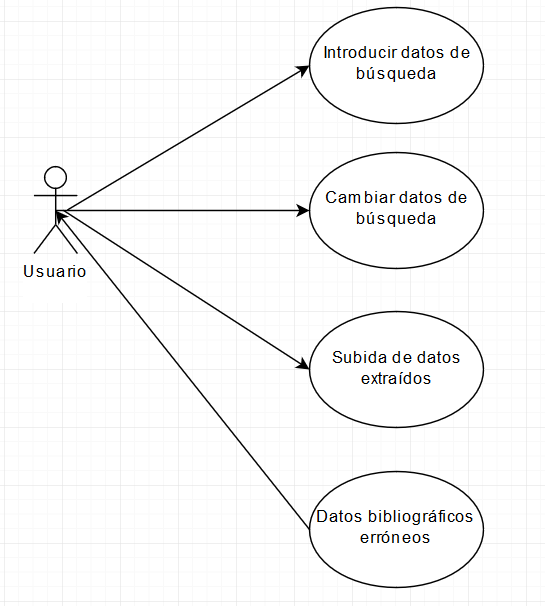
\includegraphics[width=0.8\textwidth]{UML1}
	\caption{Diagrama UML general de casos de uso.}
\end{figure}

\begin{figure}[H]
	\centering
	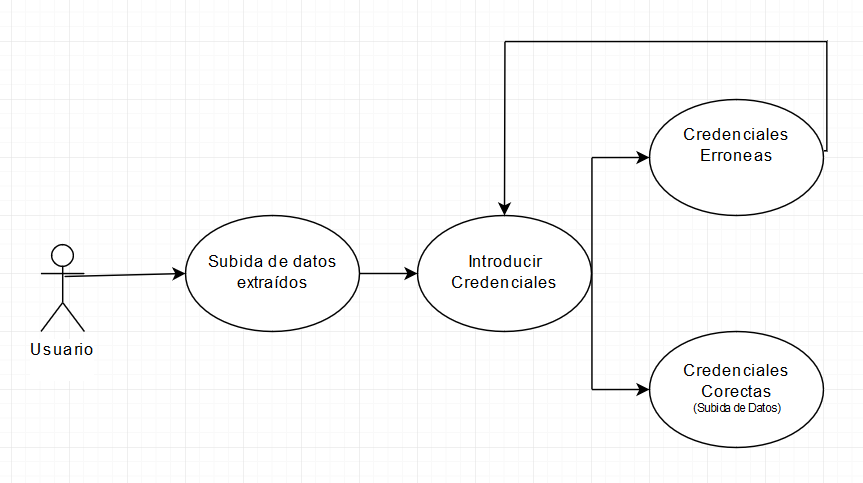
\includegraphics[width=1\textwidth]{UML2}
	\caption{Diagrama UML desglosado del caso de uso 3.}
\end{figure}

\tablaSmallSinColores{Caso de uso 1: Introducir datos de búsqueda}{p{3cm} p{.75cm} p{9.5cm}}{b1}{
	\multicolumn{3}{l}{Caso de uso 1: introducir datos de búsqueda} \\
}
{
	Descripción                            & \multicolumn{2}{p{10.25cm}}{El usuario debe introducir los datos referentes al autor a buscar} \\\hline
	\multirow{2}{3.5cm}{Requisitos}  &\multicolumn{2}{p{10.25cm}}{RF-1} \\\cline{2-3}
	\\\hline
	Precondiciones                         &   Ninguna   & 
	\\\hline
	\multirow{2}{3.5cm}{Secuencia normal}  & Paso & Acción \\\cline{2-3}
	& 1    & El usuario inicia la herramienta. 
	\\\cline{2-3}
	& 2    & El usuario introduce el nombre de autor para \emph{Google Scholar}.
	\\\cline{2-3}
	& 3    & El usuario introduce el \emph{author ID} para \emph{Scopus}.
	\\\cline{2-3}
	& 4    & El usuario introduce el nombre de autor para \emph{Web of Science}.
	\\\cline{2-3}
	& 5    & El usuario pulsa el botón \emph{Search} para comenzar la búsqueda.                                  	 
	\\\hline
	Postcondiciones                        & \multicolumn{2}{p{10.25cm}}{Se produce un cambio en la interfaz que indica al usuario que el proceso de búsqueda a comenzado} \\\hline
	Excepciones                        & \multicolumn{2}{p{10.25cm}}{Ninguna}\\\hline
	Importancia                            & Alta \\\hline
	Urgencia                               & Alta \\\hline
	Comentarios                            & & \\
}

\tablaSmallSinColores{Caso de uso 2: cambiar datos de búsqueda}{p{3cm} p{.75cm} p{9.5cm}}{b1}{
	\multicolumn{3}{l}{Caso de uso 2: Cambiar datos de búsqueda} \\
}
{
	Descripción                            & \multicolumn{2}{p{10.25cm}}{El usuario debe introducir los datos que se han introducido de forma errónea o que no han producido resultados} \\\hline
	\multirow{2}{3.5cm}{Requisitos}  &\multicolumn{2}{p{10.25cm}}{RF-1,RF-2} \\\cline{2-3}
	\\\hline
	Precondiciones                         & \multicolumn{2}{p{10.25cm}}{Se ha llevado a cabo RF-1} 
	\\\hline
	\multirow{2}{3.5cm}{Secuencia normal}  & Paso & Acción \\\cline{2-3}
	& 1    & Se detecta un error con los datos introducidos. 
	\\\cline{2-3}
	& 2    & Se muestra una nueva entrada de datos, correspondiente al proceso que se está llevando a cabo.
	\\\cline{2-3}
	& 3    & El usuario introduce los datos.
	\\\cline{2-3}
	& 4    & El proceso de búsqueda es reactivado con los nuevos datos.                                 	 
	\\\hline
	Postcondiciones                        & \multicolumn{2}{p{10.25cm}}{Se reanuda el proceso de búsqueda y se produce un cambio en la interfaz que indica al usuario que este ha sido reactivado} \\\hline
	Excepciones                        & \multicolumn{2}{p{10.25cm}}{Ninguna}\\\hline
	Importancia                            & Alta \\\hline
	Urgencia                               & Alta \\\hline
	Comentarios                            & & \\
}

\tablaSmallSinColores{Caso de uso 3: subida de datos extraídos}{p{3cm} p{.75cm} p{9.5cm}}{b1}{
	\multicolumn{3}{l}{Caso de uso 3: Subida de datos extraídos} \\
}
{
	Descripción                            & \multicolumn{2}{p{10.25cm}}{El usuario debe introducir las credenciales de acceso a ANECA, para iniciar el proceso de subida de los datos previamente extraídos } \\\hline
	\multirow{2}{3.5cm}{Requisitos}  &\multicolumn{2}{p{10.25cm}}{RF-3} \\\cline{2-3}
	\\\hline
	Precondiciones                         & \multicolumn{2}{p{10.25cm}}{Se ha llevado a cabo RF-1} 
	\\\hline
	\multirow{2}{3.5cm}{Secuencia normal}  & Paso & Acción \\\cline{2-3}
	& 1    & Se introduce las credenciales de acceso. 
	\\\cline{2-3}
	& 2    & Se comprueba que las credenciales son correctas.
	\\\cline{2-3}
	& 3    & Se activa el proceso de subida de los datos a la aplicación virtual.                               	 
	\\\hline
	Postcondiciones                        & \multicolumn{2}{p{10.25cm}}{Se  produce un cambio en la interfaz que indica al usuario que el proceso se está llevando a cabo} \\\hline
	Excepciones                        & \multicolumn{2}{p{10.25cm}}{Ninguna}\\\hline
	Importancia                            & Alta \\\hline
	Urgencia                               & Alta \\\hline
	Comentarios                            & & \\
}
\tablaSmallSinColores{Caso de uso 3.1: Credenciales erróneas }{p{3cm} p{.75cm} p{9.5cm}}{b1}{
	\multicolumn{3}{l}{Caso de uso 3.1: credenciales erróneas} \\
}
{
	Descripción                            & \multicolumn{2}{p{10.25cm}}{La herramienta debe identificar que las credenciales introducidas son erróneas y ofrecer la posibilidad de volver a introducirlas.} \\\hline
	\multirow{2}{3.5cm}{Requisitos}  &\multicolumn{2}{p{10.25cm}}{RF-3.1} \\\cline{2-3}
	\\\hline
	Precondiciones                         & \multicolumn{2}{p{10.25cm}}{Se ha llevado a cabo RF-3} 
	\\\hline
	\multirow{2}{3.5cm}{Secuencia normal}  & Paso & Acción \\\cline{2-3}
	& 1    & Se comprueba que las credenciales son erróneas \emph{.bib}. 
	\\\cline{2-3}
	& 2    & Se ofrece la posibilidad al usuario de volver a introducirlas.                              	 
	\\\hline
	Postcondiciones                        & \multicolumn{2}{p{10.25cm}}{Ninguna} \\\hline
	Excepciones                        & \multicolumn{2}{p{10.25cm}}{Ninguna}\\\hline
	Importancia                            & Alta \\\hline
	Urgencia                               & Alta \\\hline
	Comentarios                            & & \\
}

\tablaSmallSinColores{Caso de uso 3.2: Credenciales correctas }{p{3cm} p{.75cm} p{9.5cm}}{b1}{
	\multicolumn{3}{l}{Caso de uso 3.2: credenciales correctas} \\
}
{
	Descripción                            & \multicolumn{2}{p{10.25cm}}{La herramienta debe identificar que las credenciales introducidas son correctas y comenzar el proceso de subida de datos.} \\\hline
	\multirow{2}{3.5cm}{Requisitos}  &\multicolumn{2}{p{10.25cm}}{RF-3.2} \\\cline{2-3}
	\\\hline
	Precondiciones                         & \multicolumn{2}{p{10.25cm}}{Se ha llevado a cabo RF-3} 
	\\\hline
	\multirow{2}{3.5cm}{Secuencia normal}  & Paso & Acción \\\cline{2-3}
	& 1    & Se comprueba que las credenciales son correctas \emph{.bib}. 
	\\\cline{2-3}
	& 2    & Se comienza el proceso de subida de datos.                              	 
	\\\hline
	Postcondiciones                        & \multicolumn{2}{p{10.25cm}}{Cambio en la interfaz que indica al usuario que el proceso de subida se está llevando a cabo} \\\hline
	Excepciones                        & \multicolumn{2}{p{10.25cm}}{Ninguna}\\\hline
	Importancia                            & Alta \\\hline
	Urgencia                               & Alta \\\hline
	Comentarios                            & & \\
}

\tablaSmallSinColores{Caso de uso 4: Datos bibliográficos erróneos}{p{3cm} p{.75cm} p{9.5cm}}{b1}{
	\multicolumn{3}{l}{Caso de uso 4: datos bibliográficos erróneos} \\
}
{
	Descripción                            & \multicolumn{2}{p{10.25cm}}{La herramienta debe guardar e informar al usuario de los datos bibliográficos que no han podido ser subidos a ACADEMIA } \\\hline
	\multirow{2}{3.5cm}{Requisitos}  &\multicolumn{2}{p{10.25cm}}{RF-3} \\\cline{2-3}
	\\\hline
	Precondiciones                         & \multicolumn{2}{p{10.25cm}}{Se ha llevado a cabo RF-3} 
	\\\hline
	\multirow{2}{3.5cm}{Secuencia normal}  & Paso & Acción \\\cline{2-3}
	& 1    & Se almacenan los datos erróneos en un fichero \emph{.bib}. 
	\\\cline{2-3}
	& 2    & Se notifica al usuario del número de datos que no han podido ser subidos.                              	 
	\\\hline
	Postcondiciones                        & \multicolumn{2}{p{10.25cm}}{Ninguna} \\\hline
	Excepciones                        & \multicolumn{2}{p{10.25cm}}{Ninguna}\\\hline
	Importancia                            & Alta \\\hline
	Urgencia                               & Alta \\\hline
	Comentarios                            & & \\
}

\apendice{Especificación de diseño}

\section{Introducción}
En este apartado se va a explicar el porqué del diseño de los datos, la arquitectura, los procesos y la interfaz gráfica de la aplicación.\\
Lo que se pretende con este apartado es que se conozca el porqué de la toma de decisiones con respectos a los aspectos arriba comentados y los motivos que han llevado a tomar esa decisión.
\section{Diseño de datos}
Los principales datos con los que se trabaja en esta aplicación son los datos bibliográficos y como ya se explicó en la memoria, concretamente en el apartado \textbf{5.4 Formato de almacenamiento}. En ese apartado se explica que se presentaron 3 formatos alternativos para el manejo de los datos y que finalmente se acabó eligiendo el formato \emph{BibTeX} por sus etiquetas más descriptivas y su mayor facilidad de trabajo, ya que existen un gran número librerías que permiten un fácil manejo de los datos.
\section{Diseño procedimental} \label{diseño procedimental}
\begin{figure}[H]
	\centering
	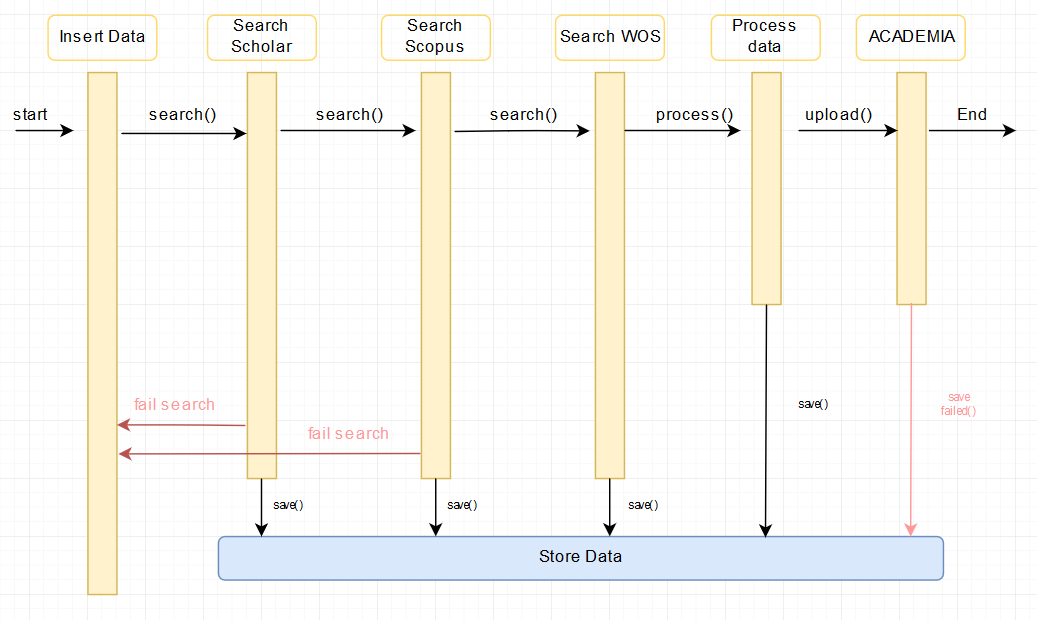
\includegraphics[width=1\textwidth]{procedimental}
	\caption{Diagrama de secuencia de la aplicación.}
	\label{fig:procedmiental}
\end{figure}

Como podemos ver en la figura \ref{fig:procedmiental} se trata de un modelo secuencial y con una sola dirección , esto se debe a que la idea que se concibió para esta aplicación es como un herramienta sencilla de fácil usabilidad pero que fuera perfectamente funcional. A continuación se va a explicar el proceso que se ve en la imagen:
\begin{enumerate}
	\item Introduce los datos referentes a la búsqueda.
	\item Se procede a la extracción de los datos en \emph{Google Scholar}, si la extracción no diera resultados el usuario sería preguntado para introducir los datos de nuevo.
	\item Se procede a la extracción de los datos en \emph{Scopus} si la extracción no diera resultados el usuario sería preguntado para introducir los datos de nuevo.
	\item Se procede a la extracción de los datos en \emph{Web of Science}
	\item Se procesan los datos
	\item Se accede a ACADEMIA y se procede a la subida de los datos resultantes del anterior paso.
	\item Los datos que no han podido ser subidos son almacenados para una posterior revisión por parte del usuario.
\end{enumerate}

\section{Diseño arquitectónico}
\subsection{Modelo-Vista-Controlador}

El Modelo-vista-controlador es un patrón de arquitectura de software, que se basa en la separación de los datos y la funcionalidad de la representación gráfica, para ello se sirve de tres componentes: modelo, vista, controlador. Lo que se persigue con este modelo es la separación de conceptos y la reutilización de código.
\begin{figure}[H]
	\centering
	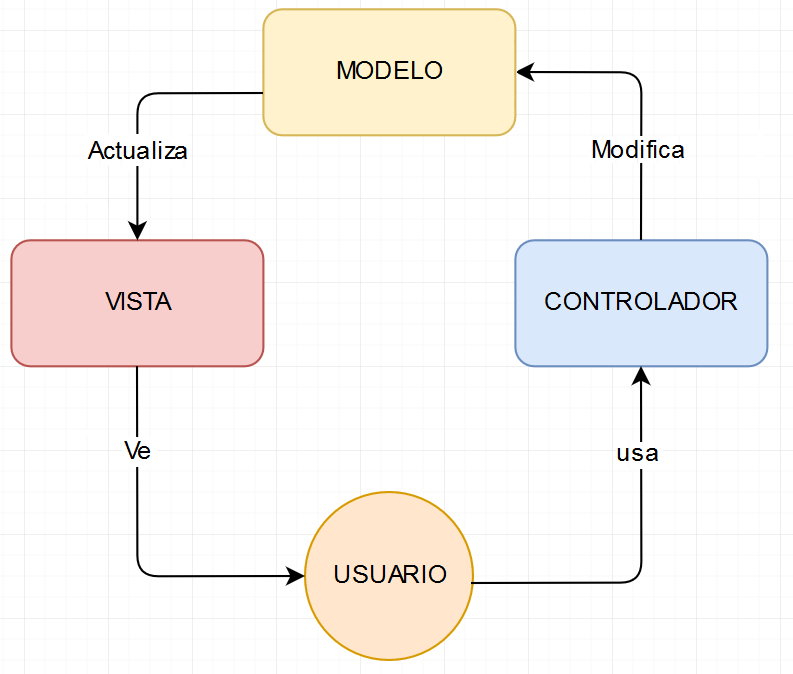
\includegraphics[width=1\textwidth]{MVC}
	\caption{Diagrama de MVC.}
	\label{fig:MVC}
\end{figure}
\begin{itemize}
	\item \textbf{Modelo.} Es la representación de la información con la cual la aplicación realiza las operaciones, es decir gestiona todos los accesos del sistema a la información. Envía a la vista la información necesaria en cada momento y que es solicitada por parte del usuario a través del controlador.
	\item \textbf{Vista.} Muestra el \emph{modelo} es decir la información, en un formato adecuado para que sea entendida por el usuario y que le permita interactuar de una manera simple y adecuada.
	\item \textbf{Controlador.} El controlador responde a los eventos fruto de la interacción del usuario con la \emph{vista} y envía peticiones al \emph{modelo} para actualizar la información en la \emph{vista}. Podemos decir que el controlador hace de intermediario entre el \emph{modelo} y la \emph{vista}
\end{itemize}

Como vemos en la figura \ref{fig:MVC}:
\begin{enumerate}
	\item El usuario interactúa con la vista.
	\item El controlador recibe una petición de acción.
	\item El controlador realiza las peticiones para la modificación del modelo.
	\item El modelo envía la nueva información a mostrar a la vista.
	\item La vista se encarga de mostrar la información de la manera adecuada.
	\item El usuario ve la nueva información y empieza de nuevo el proceso.
\end{enumerate}
\subsection{Arquitectura General}
La arquitectura general de la aplicación vista de una forma simplificada sería:
\begin{figure}[H]
	\centering
	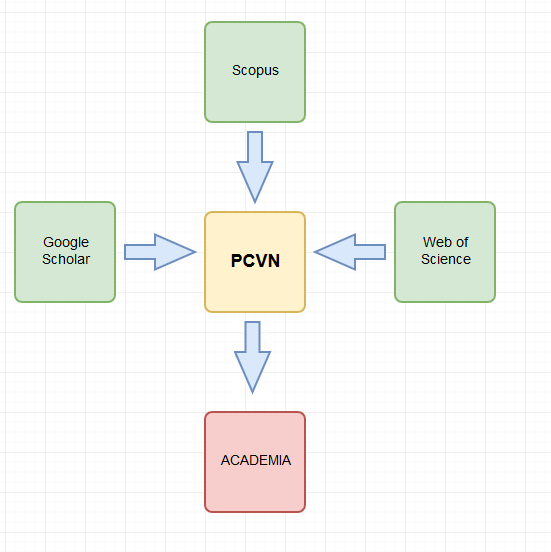
\includegraphics[width=0.8\textwidth]{esquema}
	\caption{Arquitectura de la aplicación.}
	\label{fig:esquema}
\end{figure}
Como vemos en la sección \ref{fig:esquema} se efectúa todo el proceso de manera secuencial, se extraen los datos , se procesan y modelan adecuadamente y finalmente se suben a ACADEMIA como se ha explicado en \ref{diseño procedimental}
\section{Diseño de interfaces}
Para el diseño de la interfaz se buscaba sencillez y funcionalidad, dos requisitos que se han solventado con el uso de la librería para \emph{Python} \emph{Tkinter}, la cual ofrece funcionalidades más que suficientes y un uso sencillo y eficaz.

Con el fin de mejorar la experiencia del usuario con el uso de la interfaz se han integrado una serie de contenedores de texto y barras de progreso que: 
\begin{itemize}
	\item Informan al usuario de la tarea que se está llevando a cabo y de qué es lo que pasará después.
	\item Informa al usuario del progreso de la tarea y cuánto falta para la finalización de esta.
\end{itemize}

A continuación vamos a ver unas imágenes de ejemplo de cómo se ve esta interfaz.
\begin{figure}[H]
	\centering
	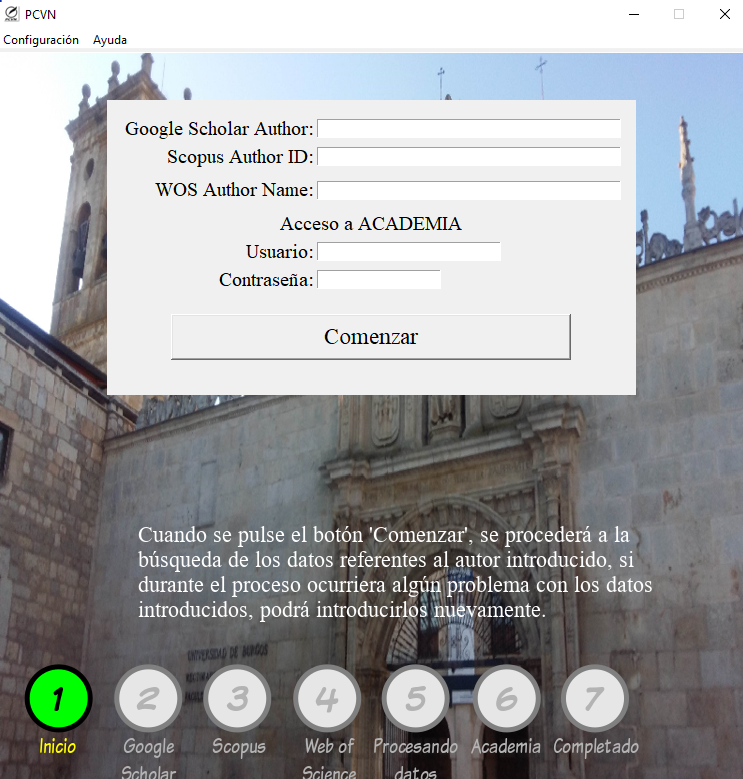
\includegraphics[width=1\textwidth]{GUI1}
	\caption{Imagen de ejemplo de la interfaz gráfica.}
	\label{fig:gui1}
\end{figure}
Vemos en la figura \ref{fig:gui1} una interfaz simple y sencilla, sin objetos agresivos o intrusivos.
\begin{figure}[H]
	\centering
	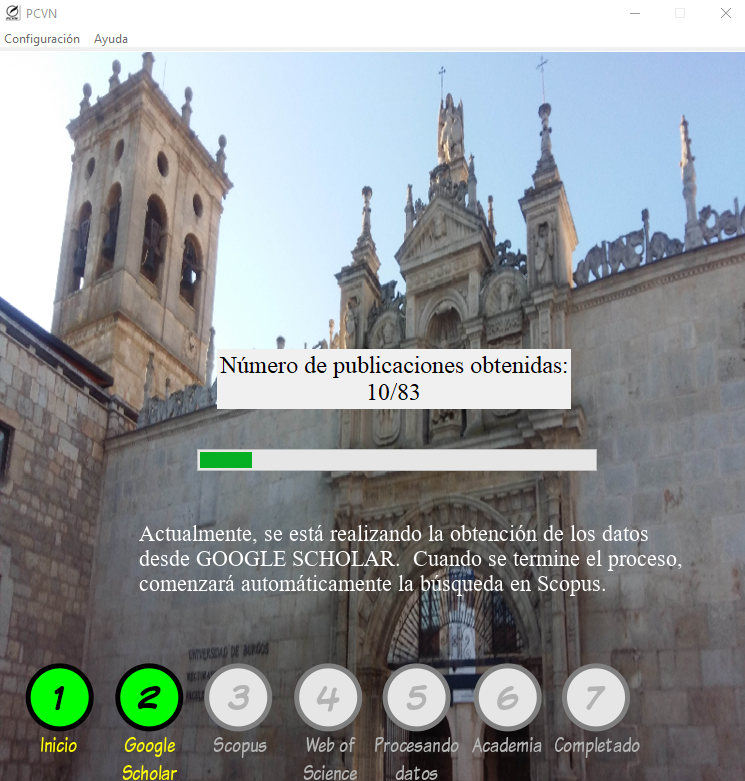
\includegraphics[width=1\textwidth]{GUI2}
	\caption{Imagen de ejemplo de la interfaz gráfica.}
	\label{fig:gui2}
\end{figure}

Vemos en la figura \ref{fig:gui2} como en todo momento el usuario es informado de lo que está pasando y del estado de la tarea.

Se ha utilizado una gama de colores suaves y un fondo sobrio y elegante para conservar el corte simplista y estético de la aplicación que hace que los textos importantes sea lo que más llame la atención al usuario.

El único momento en el que se han utilizado colores fuertes y llamativos es cuando el usuario introduce erróneamente los datos, esto es para informar al usuario de que es lo que debe corregir como vemos en la figura \ref{fig:gui4} 
\begin{figure}[H]
	\centering
	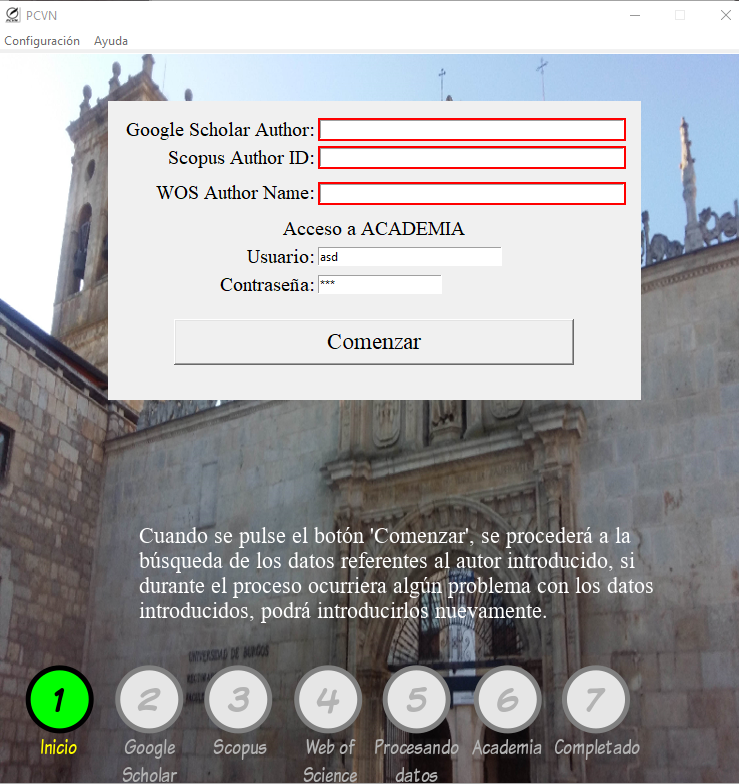
\includegraphics[width=1\textwidth]{GUI4}
	\caption{Imagen de ejemplo de error en la interfaz gráfica.}
	\label{fig:gui4}
\end{figure}

Para informar al usuario de errores acontecidos durante la normal ejecución de la aplicación se han utilizado ventanas emergentes que captan la atención del usuario y lo hacen centrarse en el mensaje que este transmite como se puede ver en la  figura \ref{fig:gui3}
\begin{figure}[H]
	\centering
	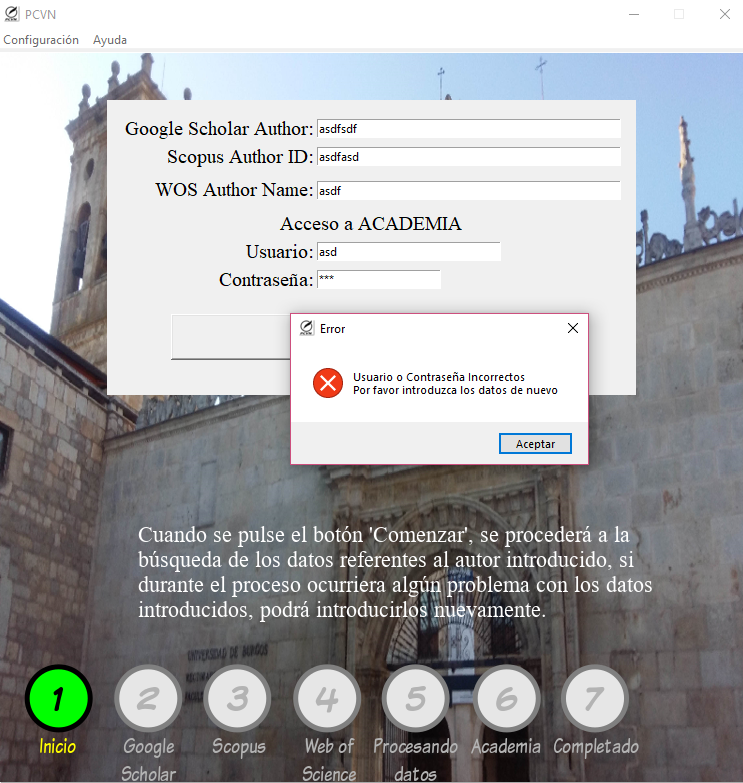
\includegraphics[width=1\textwidth]{GUI3}
	\caption{Imagen de ejemplo de ventana emergente.}
	\label{fig:gui3}
\end{figure}

\apendice{Documentación técnica de programación}

\section{Introducción}

\section{Estructura de directorios}

\section{Manual del programador}

\section{Compilación, instalación y ejecución del proyecto}

\section{Pruebas del sistema}

\apendice{Documentación de usuario}
\section{Introducción}
En este apartado se van a detallar los pasos necesarios para ejecutar la aplicación desde el punto de vista del usuario.
\section{Requisitos de usuarios}
Los requisitos mínimos para poder hacer uso de la aplicación son:
\begin{itemize}
	\item Tener instalado \emph{Python 3}
	\item Tener instalado las librerías correspondientes (\emph{Scholarly, Bibtexparser, Selenium, PIL}).En el anexo \ref{instalar} se especifica como se pueden obtener estas librerías.
	\item Disponer de conexión a Internet.
	\item Disponer de acceso a los recursos científicos del \emph{FECYT}, para ello valdría acceso a la red de la universidad o bien una VPN a esta red si se pretende trabajar desde casa.
	\item Cuenta registrada en la aplicación web ACADEMIA. para ello basta con acceder al enlace \cite{registro} y cumplimentar los datos de registro.
\end{itemize}
\section{Instalación}
Para la ejecución de la aplicación no es necesario una instalación tradicional del proyecto, simplemente es necesario clonar o descargar el repositorio desde \emph{GitHub} y ejecutarlo como se ha indicado en el Anexo \ref{ejecutar}
\section{Manual del usuario}
A continuación, vamos a explicar los pasos a seguir por parte de un usuario cualquiera para un correcto uso de la aplicación.

\subsection{Introducción de datos}
Nada más ejecutar la aplicación se nos presentará la siguiente interfaz:
\begin{figure}[H]
	\centering
	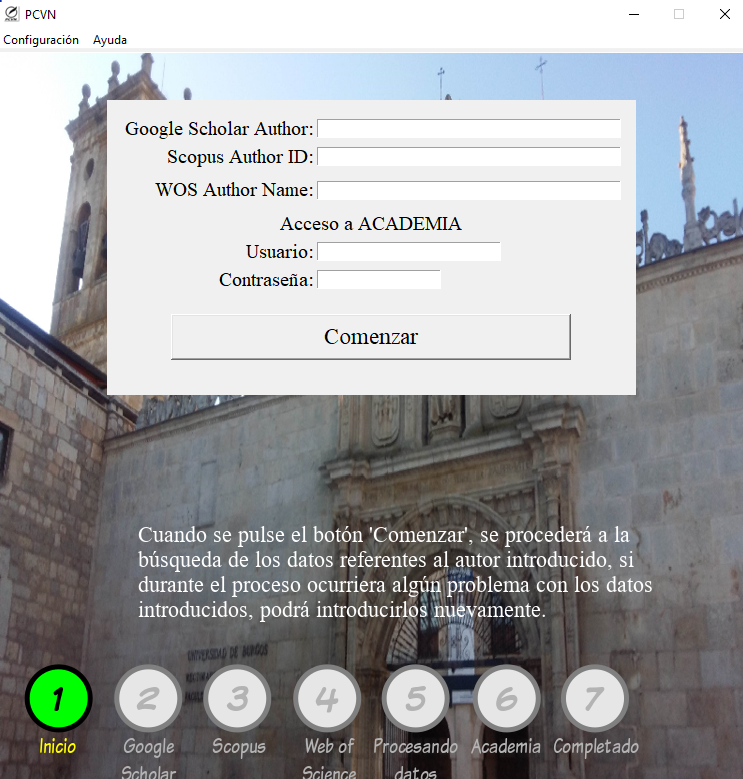
\includegraphics[width=0.8\textwidth]{GUI1}
	\caption{Imagen de ejemplo de uso.}
\end{figure}
en la que como vemos existen una serie de recuadros donde se ha de introducir el identificador para cada una de las páginas (Nombre, ID, Nombre, Usuario y contraseña). En el cuadro de texto de la parte inferior observamos que se nos indica que es lo que va a suceder a continuación. Esto sería un uso completo de la aplicación, es decir se buscan las publicaciones de un autor, se procesan y con las credenciales introducidas por el usuario se suben a su cuenta de ACADEMIA. Sin embargo, con el menú desplegable que podemos ver en la parte superior de la imagen podemos cambiarlo, este menú nos permite:
\begin{itemize}
	\item Configurar el número máximo de publicaciones que queremos extraer.
	
	\begin{figure}[H]
	\centering
	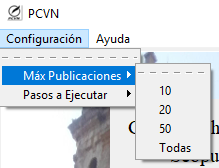
\includegraphics[width=0.5\textwidth]{GUI_menu1}
	\caption{Imagen configuración de publicaciones.}
	\end{figure}
	
	\item Configurar que procesos queremos llevar acabo. La opción por defecto es el uso completo de la aplicación, si bien podemos elegir cual de los procesos se quiere llevar a cabo. Según sea nuestra elección se nos cambiará a una u otra ventana y se adaptaran los textos informativos para informarnos fielmente de lo que va a ocurrir.
	
	\begin{figure}[H]
	\centering
	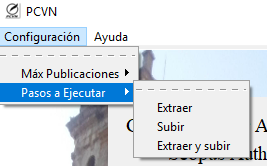
\includegraphics[width=0.5\textwidth]{GUI_menu2}
	\caption{Imagen configuración de procesos a ejecutar.}
	\end{figure}
	
	\item Ayuda, que nos abrirá un documento \emph{pdf} que ofrece ayuda sobre el correcto uso de la aplicación.
\end{itemize}

Vamos a seguir la ejecución completa del proceso pues engloba el resto de opciones a elegir.\\ Una vez introducidos los datos pulsamos sobre el botón \emph{Comenzar}. Entonces se producirá un cambio en la interfaz que indica que se está procediendo a la extracción de datos.
En este punto pueden ocurrir 2 cosas:

\begin{itemize}
	\item Todo vaya según lo previsto, entonces se mostrará una interfaz como la siguiente:
	\begin{figure}[H]
	\centering
	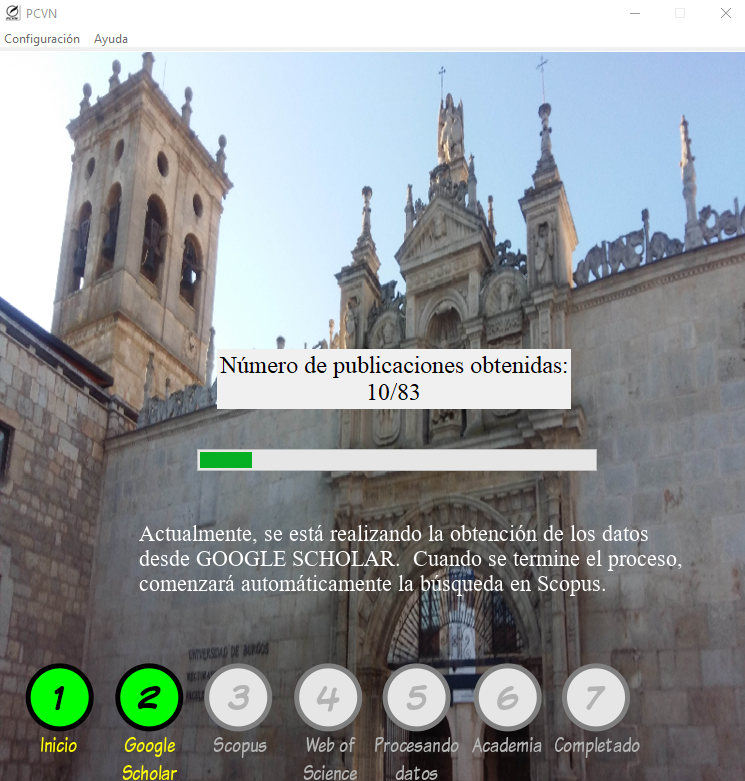
\includegraphics[width=0.8\textwidth]{GUI2}
	\caption{Imagen de extracción de información de \emph{Google Search}.}
	\end{figure}
	Una vez completada la barra saltará al siguiente proceso.
	\item Exista algún problema con la ejecución, por ejemplo, no se disponga de conexión a Internet o los datos introducidos para el autor no generan ningún resultado. Entonces se mostrará la siguiente interfaz:
		\begin{figure}[H]
	\centering
	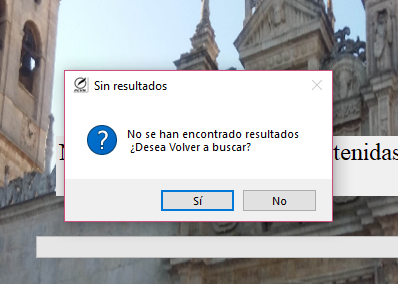
\includegraphics[width=0.6\textwidth]{GUI_error_gs}
	\caption{Imagen de error en el proceso de búsqueda de \emph{Google Search}.}
	\end{figure}
	Dependiendo del error que se haya producido (Sin conexión, Sin resultados, etc.) se mostrará un mensaje u otro en la ventana emergente.Ahora volvemos a tener dos opciones:
	\begin{itemize}
		\item Volver a introducir los datos referentes al autor, pero esta vez únicamente para \emph{Google Search}. como vemos en la siguiente imagen.
		\begin{figure}[H]
	\centering
	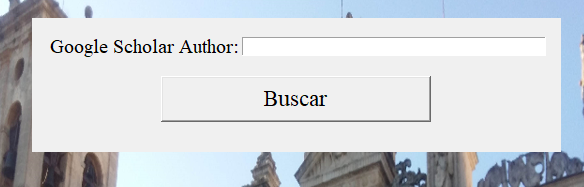
\includegraphics[width=0.8\textwidth]{gui_scholar_resch}
	\caption{Imagen de vuelta a buscar en \emph{Google Search}}
	\end{figure}
		\item Finalizar aquí la ejecución de la aplicación.
	\end{itemize}
\end{itemize}

Una vez finalizado el proceso anterior correctamente se procederá automáticamente a realizar la extracción de los datos de \emph{Scopus} con un nuevo cambio en la interfaz y donde nos puede ocurrir algo similar a lo acontecido en el paso anterior:
\begin{itemize}
	\item Todo vaya según lo previsto con lo que se procederá a la extracción de los datos.
	
	\begin{figure}[H]
	\centering
	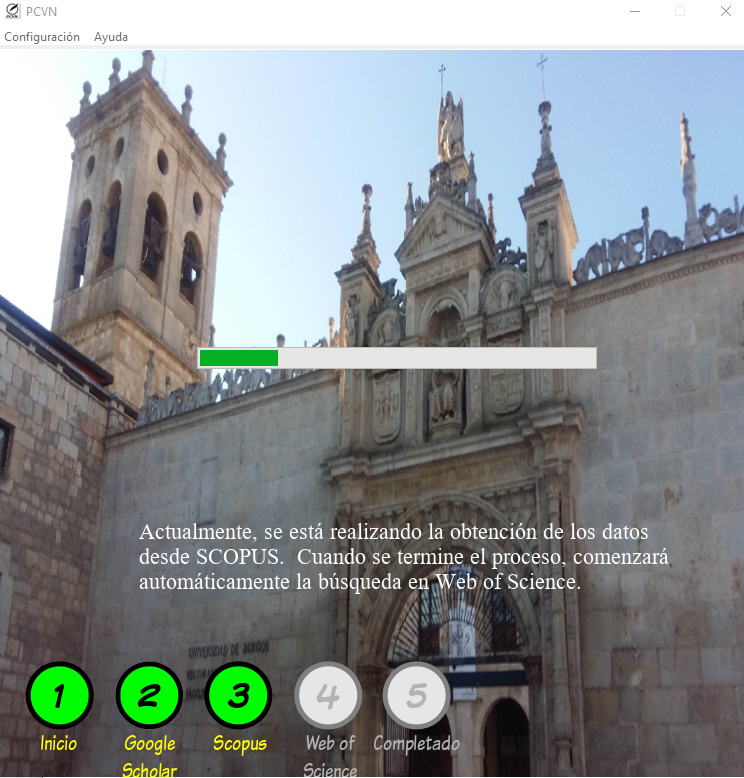
\includegraphics[width=0.8\textwidth]{GUI_scopus}
	\caption{Imagen de búsqueda en \emph{Scopus}}
	\end{figure}
	
	\item Que se detecte algún problema con los datos o la conexión, lo que termine en una nueva introducción de datos.
	
	\begin{figure}[H]
	\centering
	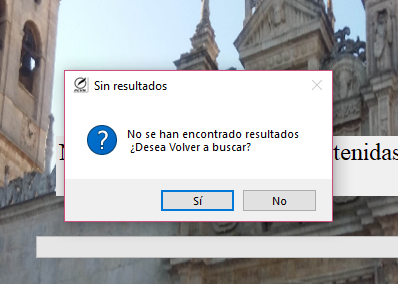
\includegraphics[width=0.8\textwidth]{GUI_error_gs}
	\caption{Imagen de error en el proceso de búsqueda de \emph{Scopus}.}
	\end{figure}
	
	Aquí se nos vuelven a presentar una serie de opciones:
	\begin{itemize}
		\item Volver a introducir los datos referentes al autor 
			
		\begin{figure}[H]
		\centering
		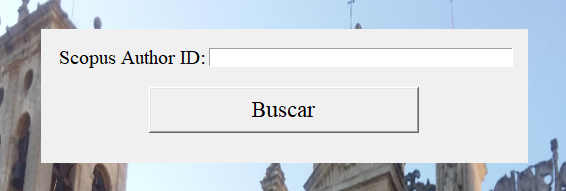
\includegraphics[width=0.8\textwidth]{gui_scopus_rsch}
		\caption{Imagen de volver a buscar en \emph{Scopus}.}
		\end{figure}
	
		\item Finalizar aquí la ejecución de la aplicación.
		\item En el caso de que se haya tratado de otro tipo de error (de conexión , error interno ,etc.) se podrá reintentar el proceso con los mimos datos.
	\end{itemize}
\end{itemize}
Una vez finalizado este proceso correctamente automáticamente habrá un cambio en la interfaz que indica que se ha procedido con el siguiente proceso de extracción exactamente igual que en los pasos anteriores, donde nos puede ocurrir:
\begin{itemize}
	\item Todo vaya según lo previsto con lo que se procederá a la extracción de los datos.
				
		\begin{figure}[H]
		\centering
		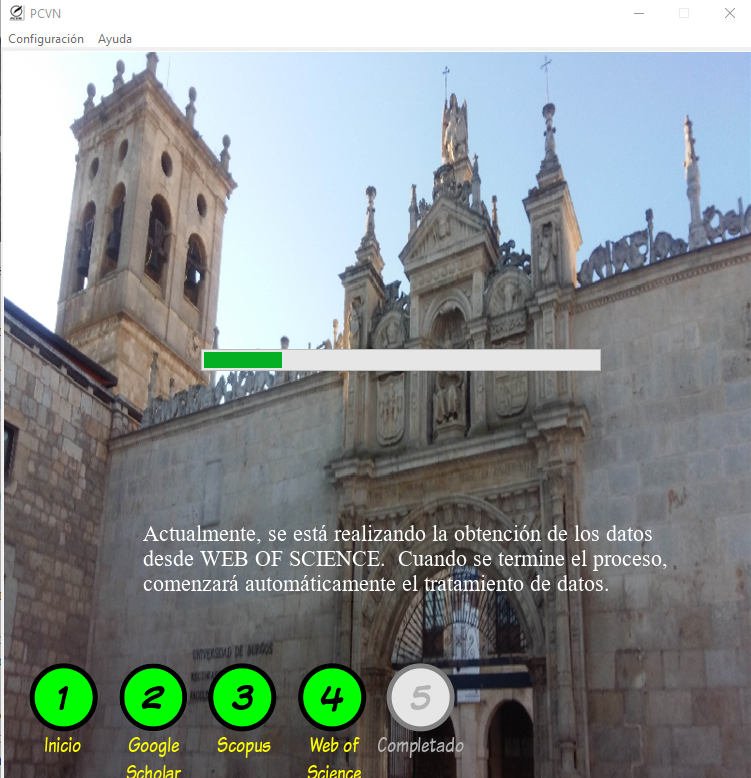
\includegraphics[width=0.8\textwidth]{GUI_wos}
		\caption{Imagen de extracción de información de\emph{Web of Science}.}
		\end{figure}
	
	\item Que se detecte algún problema con los datos o la conexión, lo que termine en una nueva introducción de datos.
		
	\begin{figure}[H]
	\centering
	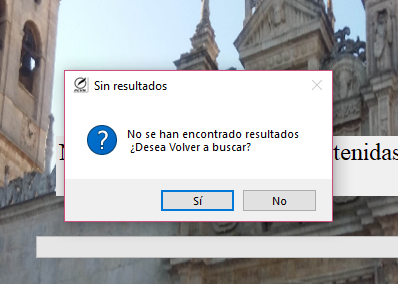
\includegraphics[width=0.8\textwidth]{GUI_error_gs}
	\caption{Imagen de error en el proceso de búsqueda de \emph{Web of Science}.}
	\end{figure}
	Aquí se nos vuelven a presentar una serie de opciones:
	\begin{itemize}
		\item Volver a introducir los datos referentes al autor 
			
		\begin{figure}[H]
		\centering
		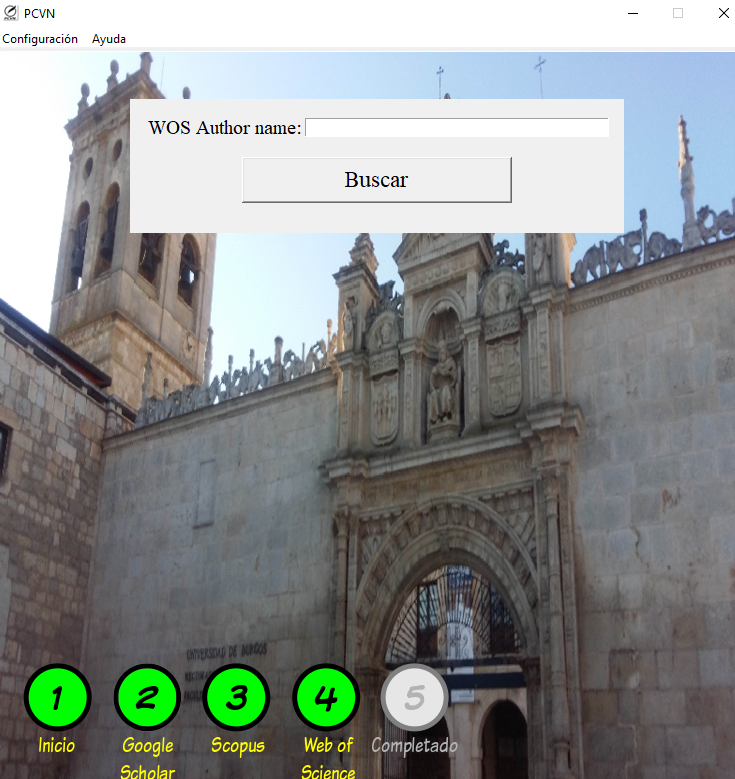
\includegraphics[width=0.8\textwidth]{gui_wos_rsch}
		\caption{Imagen de volver a buscar en \emph{Web of Science}.}
		\end{figure}
	
		\item Finalizar aquí la ejecución de la aplicación.
		\item En el caso de que se haya tratado de otro tipo de error (de conexión , error interno ,etc.) se podrá reintentar el proceso con los mimos datos.
	\end{itemize}
\end{itemize}

Cuando esta última extracción haya concluido se procederá al tratamiento de datos,	en donde simplemente habrá que esperar a que termine el proceso. Para ayudar en la visualización del progreso como en el resto de las partes de la interfaz se dispone de una barra de progresos que indica la carga de trabajo realizada.

		\begin{figure}[H]
		\centering
		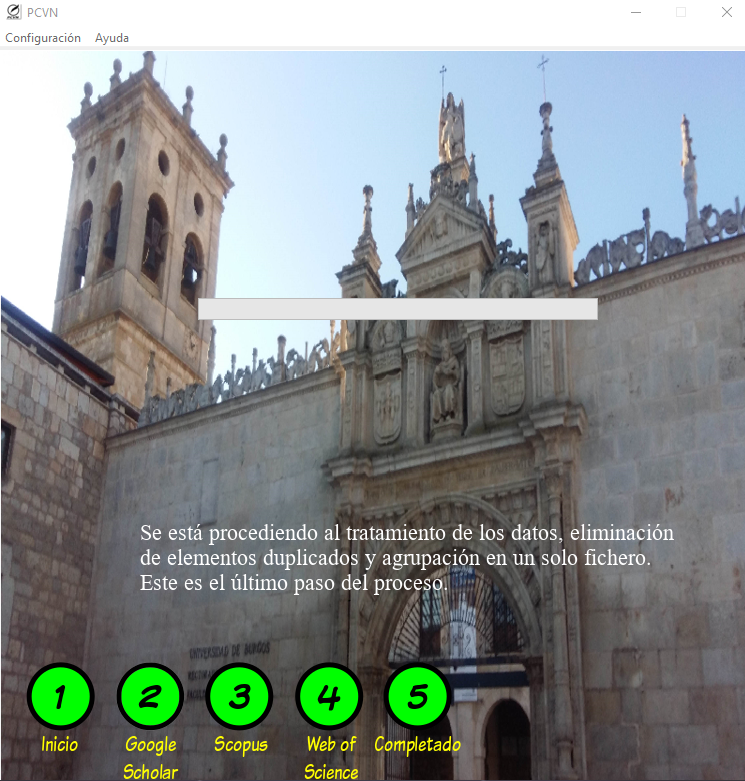
\includegraphics[width=0.8\textwidth]{GUI_procesado}
		\caption{Imagen del procesado de datos.}
		\end{figure}
		
En el caso de que se haya decidido realizar únicamente el proceso de extracción de los datos, este habría sido el último paso del proceso y se nos abriría una ventana que nos permitiría ver las publicaciones que hayan sido extraídas o bien finalizar completamente la aplicación como se ve en la siguiente imagen:

		\begin{figure}[H]
		\centering
		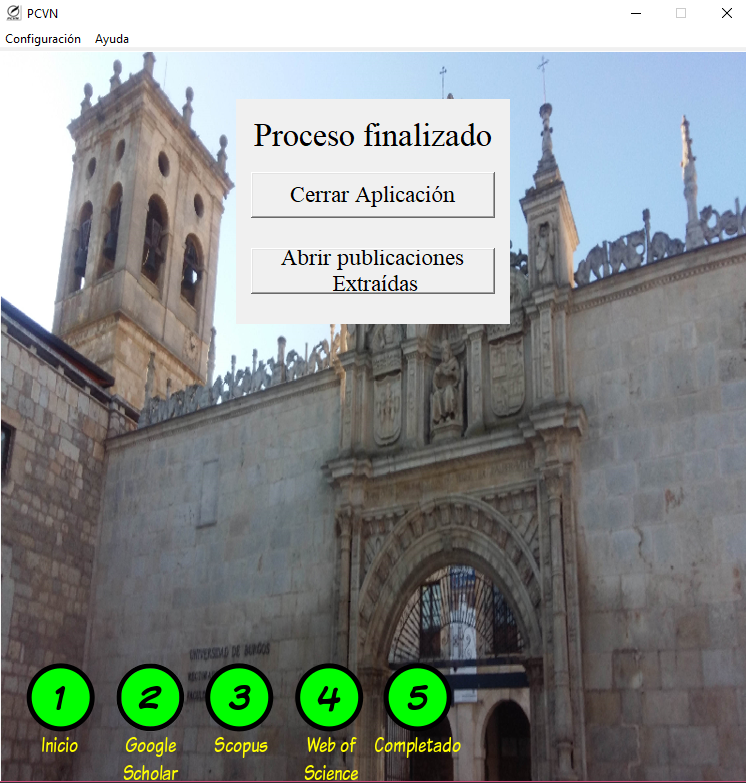
\includegraphics[width=0.8\textwidth]{GUI_fin_extr}
		\caption{Imagen final del proceso de extracción datos.}
		\end{figure}
		
En el caso de que se haya decido saltar el proceso de extracción de datos y se haya decidido realizar solo la subida de los datos (aportando el fichero con las publicaciones a subir), se mostrará una nueva interfaz donde se deberá introducir el nombre del autor, el usuario (DNI,NIE) y la contraseña para poder acceder a la plataforma y que comience el proceso de subida de los datos previamente extraídos. Como se puede ver en la siguiente imagen:
			
		\begin{figure}[H]
		\centering
		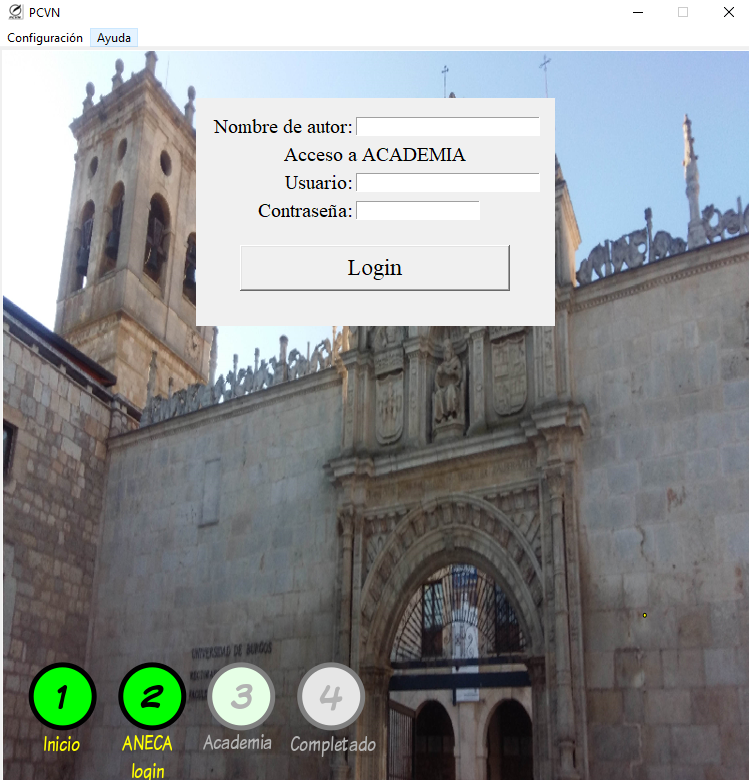
\includegraphics[width=0.8\textwidth]{GUI_login}
		\caption{Imagen de inicio de sesión.}
		\end{figure}
	

De nuevo pueden ocurrir dos cosas:
\begin{itemize}
	\item El usuario y contraseña sean correctos, con lo que se procederá con normalidad.
	\item El usuario y contraseña no sean correctos, por lo volverán a ser solicitados.
\end{itemize}
En el caso de que se haya decidido realizar el proceso completo (extracción y subida) no será necesaria la identificación pues ya se ha realizado al inicio del proceso y seguiríamos directamente con el proceso de subida de los datos. \\

Una vez debidamente identificado en la aplicación ACADEMIA se comenzará la subida de datos. De nuevo tendremos una barra de progreso que nos indica el progreso respecto del total y un cuadro de texto que nos indica que tipo de publicación se está subiendo y el número respecto el total.

		\begin{figure}[H]
		\centering
		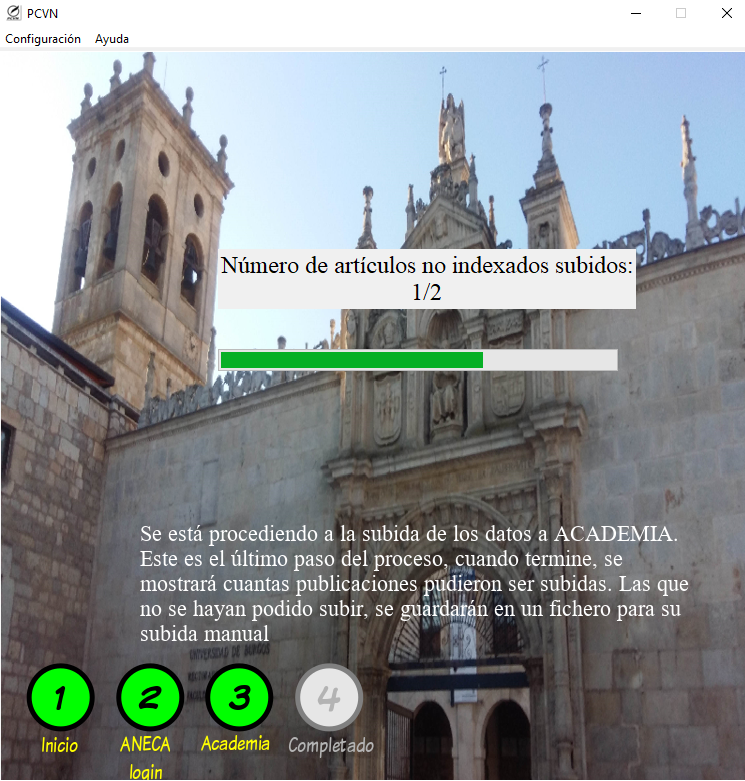
\includegraphics[width=0.8\textwidth]{GUI_subida}
		\caption{Imagen del proceso de subida.}
		\end{figure}


Para finalizar se nos muestra una pantalla final con información del número total de publicaciones y el número de publicaciones que por error de formato no han podido ser subidas. Estas publicaciones no se perderán si no que han sido guardadas en un fichero específico para una posterior revisión por parte del usuario.

		\begin{figure}[H]
		\centering
		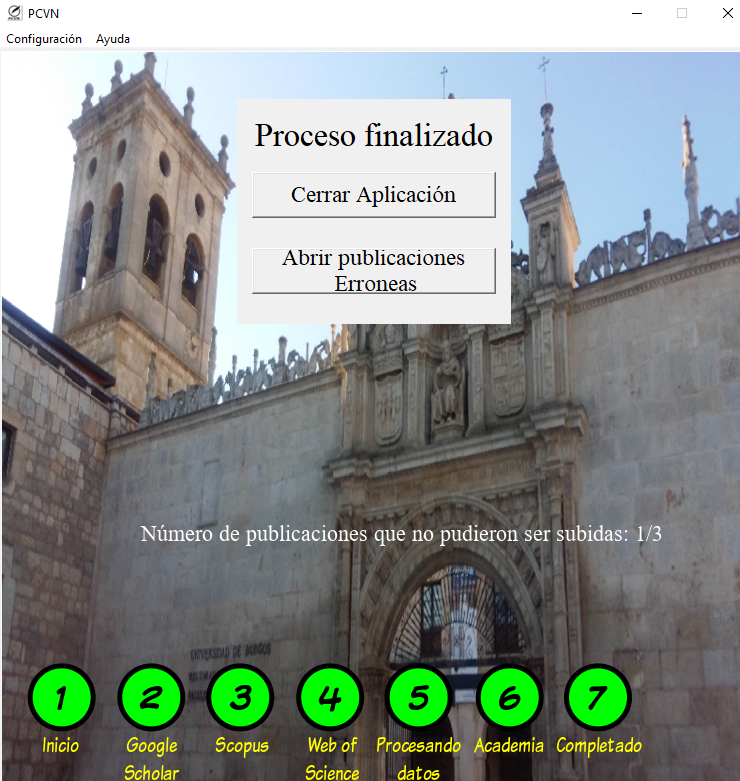
\includegraphics[width=0.8\textwidth]{GUI_completado}
		\caption{Imagen final del proceso de subida.}
		\end{figure}




\bibliographystyle{plainnat}
\bibliography{bibliografiaAnexos}

\end{document}
